\documentclass[10pt,twocolumn]{article}
\usepackage{graphicx}    % For including images
\usepackage{amsmath}     % For mathematical symbols
\usepackage{caption}     % Better captions
\usepackage{float}       % Precise float placement
\usepackage{geometry}    % To adjust margins
\geometry{margin=1in}
\usepackage[backend=biber,style=apa]{biblatex}
\addbibresource{references.bib}  % This is your .bib file name

\title{\textbf{Machine Learning-Based Classification of Table Tennis Swings Using Racket Kinematics}}
\author{Jevi Waugh \\
Faculty of Engineering, Architecture and Information Technology \\
COMP4702 - Machine Learning}
\date{May 2025}

\begin{document}

\maketitle

\begin{abstract}
This report investigates the application of machine learning models to classify the demographics of table swings based on racket kinematics data, with a strong focus on predicting a combined age and gender label. The Data Set originally sourced from DRYAD has slightly been modified for the purpose of this report. We apply and compare three supervised classification algorithms, K-Nearest Neighbors (KNN), Support Vector Machines (SVM) and One-vs-Rest Logistic Regression, evaluating their performance using known evaluation metrics. Our findings provide insights into the discriminative power of racket motion features and the behavior of various classifiers on a real-word problem.
\end{abstract}

\section{Introduction}
Human motion analysis and dexterity is a core area of research in sports, particularly in table tennis. In the context of table tennis, it is important to understand how swing patterns relate to certain demographic attributes such as age and gender, which can inform training strategies and biomechanical insights such as angular velocity, acceleration, power spectral density, etc. This report explores the use of supervised machine learning models to classify a composite label consisting of age and gender from the table tennis-racket-swing dataset. Pre-Processing will be required to ensure that valid numerical data are utilised efficiently. The considered ML models: K-Nearest Neighbor (K-NN), logistic regression and kernel based methods (such as a support vector machine) will be used. The purpose of this report is not to only maximise accuracy and lower $E_{new}$, but to primarily make a critical evaluation of each model's behavior, generalisation capability, feature proccessing, and sensitivity to hyper-parameters.

\section{Exploratory Data Analysis}
The provided dataset had some irregularities in terms of feature values and also had other inconsistencies with our classification task. The features that were dropped are 'id' and 'date' primarily because ID identifies and metadata impertinent to the player kinematics will strictly skew the classification workflow as they are strictly not-relevant to the problem.
\subsection{Encoding and Normalisation}
Our classification problem will make use one-hot-encoding for features in Table~\ref{tab:cat-values} excluding "???".  Age encodes,  low $\rightarrow$ 0, medium $\rightarrow$ 1, high $\rightarrow$ 2. This provides us the following 6 labels as shown in Table~\ref{tab:encoding-scheme}. 
We then represent these modalities as low $\rightarrow$ Young, medium $\rightarrow$ Mid-age, high $\rightarrow$ Older.
For gender, we have binary numerical values which we interpret as, 0 $\rightarrow$ Female, and 1 $\rightarrow$ Male. 
\footnote{Note that we do not encode gender but rather interpret it. Same for age but we encode once and the interpret using known terminology}
\begin{table}[H]
\centering
\caption{Encoding scheme for combined gender and age classification}
\begin{tabular}{|l|}
\hline
\textbf{Combined Labels} \\
\hline
00 $\rightarrow$ Young Female \\
10 $\rightarrow$ Young Male \\
01 $\rightarrow$ Mid-age Female \\
11 $\rightarrow$ Mid-age Male \\
02 $\rightarrow$ Older Female \\
12 $\rightarrow$ Older Male \\
\hline
\end{tabular}
\label{tab:encoding-scheme}
\end{table}
The dataset will be either normalised using the formula $x_{ij}^{new} = {\dfrac {x_{ij} - min_l{(x_{lj})}} {max_l{(x_{lj})} - min_l{(x_{lj})}}}$ or standardised, using   $Z={\dfrac {\bar{X} - \mu} {\sigma}}$depending on the model's sensitivity to feature scaling and the distribution of the data.
\subsection{Dataset description and assumptions}
\label{subsec:dataset-description-and-assumptions}
The dataset has 97,355 data-points and 49 features excluding 'id' and 'date'. There were other inconsistencies such as missing values labelled as "???" in certain columns (see Table~\ref{tab:cat-values}). There were 5 missing data points in each random variable (feature), 20 values, a total of which their rows were dropped. We also assume that the dropped rows won't affect prediction accuracy given that its only $5.13 \times 10^{-5}$\% of the entire data set.

\begin{table}[H]
\centering
\caption{Categorical values (before cleaning)}
\begin{tabular}{|l|l|}
\hline
\textbf{Feature} & \textbf{Unique Values} \\
\hline
Height     & \texttt{high, low, medium, ???} \\
Age        & \texttt{high, medium, ???, low} \\
Play Years & \texttt{high, medium, ???, low} \\
Weight     & \texttt{high, medium, low, ???} \\
\hline
\end{tabular}
\label{tab:cat-values}
\end{table}
Furthermore, an analysis on class imbalance was made to ensure full interpretability when we make predictions. We can see that in Figure~\ref{fig:stacked-results} gender has a class imbalance of 60-40\%.To address the class imabalance in gender, we will use the stratify parameter in Sciki-learn's \texttt{train\_test\_split}
 function to ensure that proportion of each class is preserved in both the training and test sets. Without stratification, random splitting of the data might over-represent one class leading to a biased model. While this imbalance is not as extreme as  presented ones such as Figure~\ref{fig:stacked-hand-results}, this ensures a much more accurate model. Handedness and holdRacketHanded both have an exact imabalance of 83-16\%. We will address this later during feature selection.

\begin{figure}[H]
    \centering
    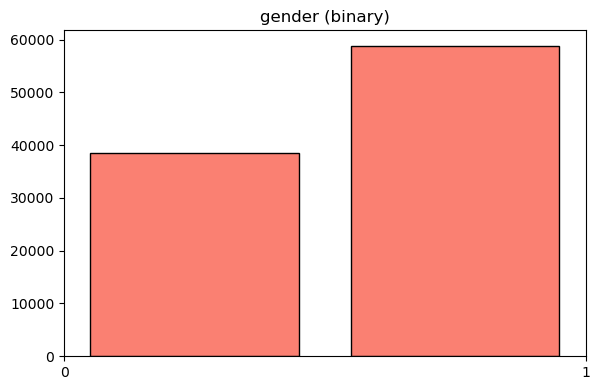
\includegraphics[width=0.85\linewidth]{gender.png}
    \caption{Gender Imbalance}
    \label{fig:stacked-results}
\end{figure}

\begin{figure}[H]
    \centering
    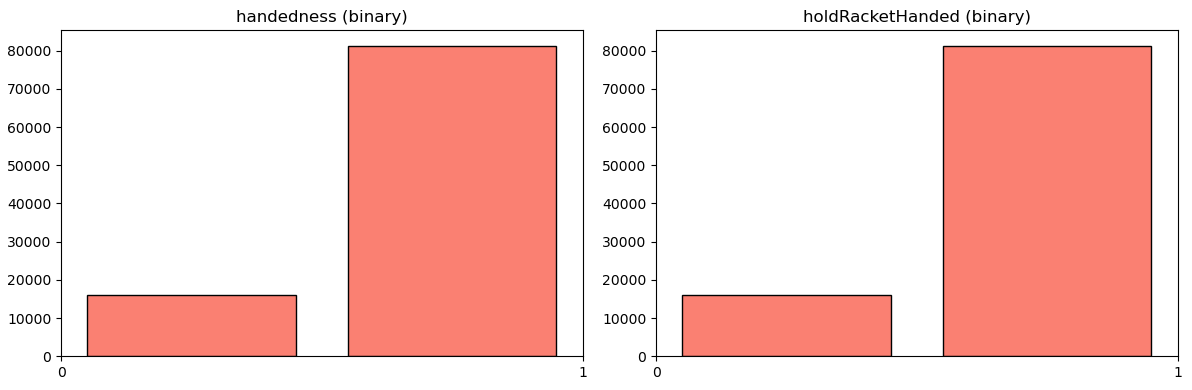
\includegraphics[width=0.85\linewidth]{hand_data.png}
    \caption{Hand data Imbalance}
    \label{fig:stacked-hand-results}
\end{figure}

We also observe the distributions of each numerical feature in the figures in the appendix, where the general assumption is that most features do not come from a normal distrbution as, most features are skewed to the right and others look uniform. Features such as \texttt{newv1}, \texttt{newv2} and \texttt{g\_max} appear to follow a Gaussian distribution, however, we cannot assume normality without statistical validation. The Central Limit Theorem suggests that convergence to a Gaussian distribution as $n \rightarrow \infty $. This is only aymptotic and does not guarantee Gaussianity in our given finite samples. Hence we will make the assumption that the dataset comprises a mixture of distributions, especially since this is a finite sample and not on the behaviour as $n \rightarrow \infty$

Before applying any machine learning model, we will indentify potential redundancy among features by computing a Pearson correlation matrix as seen in Figure~\ref{fig:correlation-matrix}
\begin{figure}[H]
    \centering
    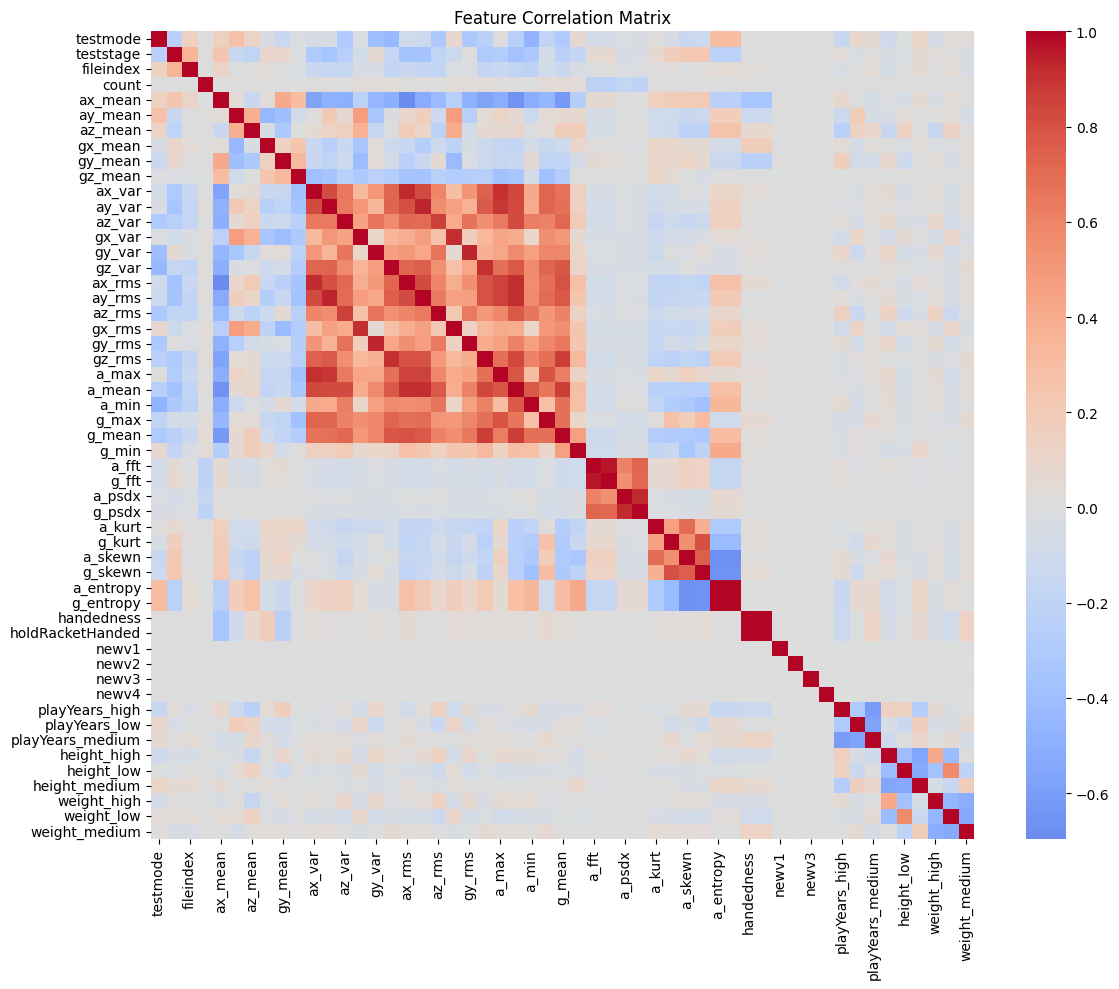
\includegraphics[width=0.85\linewidth]{correlation_matrix.png}
    \caption{Pearon's correlation matrix}
    \label{fig:correlation-matrix}
\end{figure}
We can see that the acceleration, velocity and gyro-signal features are heavily correlated. Highly correlated features can introduce multicollinearity which can negatively impact a model that assumes feature independence such as (Logistic regression). Dropping highly correlated features will be further explored in other models to evaluate its effectiveness and generalisation.

\section{Model 1: K-Nearest Neighbors (KNN)}
\subsection{Model Training and Hyper-parameter tuning}

\subsection{Accuracy and classification}
\subsection{Evaluation Metrics and Results}
\subsubsection{Accuracy and $E_{new}$ evaluation}
\subsubsection{Confusion Matrix}
\subsubsection{ROC Curves}
\subsubsection{Cross validation and learning curve}

\section{Model 2: Logistic regression}
\subsection{Solver and Regularisation Comparison}
\subsection{Feature Importance via Coefficients}
\subsection{Evaluation Metrics and Results}
\subsection{Cross validation and learning curve}
\subsection{PCA}
\subsection{Feature selection and correlation}

\section{Model 3: Support Vector Machine (SVM)}
\subsection{Kernel and regularisation exploration}
\subsection{Evaluation Metrics and Results}
\subsection{Training on non-feature selection}
This time we will explore deeper by training on a the original dataset which is highly correlated along some features and we will use a different kernel.

\section{Comparative Analysis}
\subsection{Summary Table of Model Performance}

\subsection{Bias variance tradeoff}

\subsection{Feature Sensitivity and Interpretability}


\section{Conclusion}
\subsection{Summary of Findings}
\subsection{Insights on applied models}


\clearpage  % or \newpage
\appendix
\section*{Appendix}

\begin{figure}[H]
    \centering
    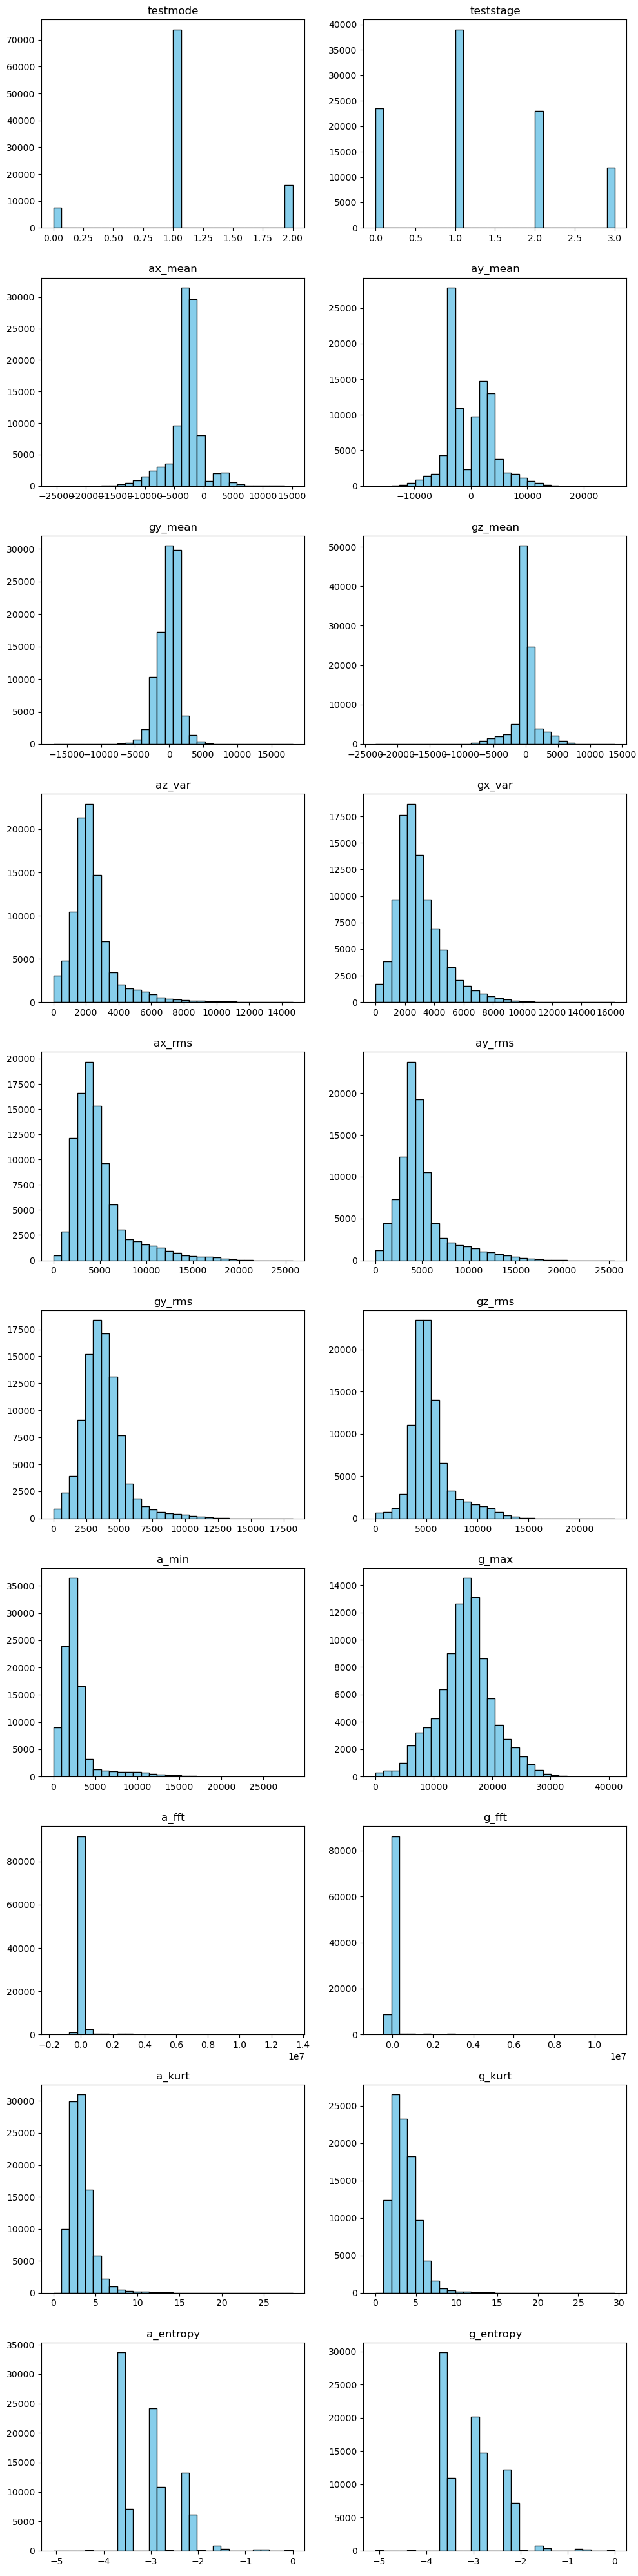
\includegraphics[width=0.85\linewidth, height=0.9\textheight]{distribution_1.png}
    \caption{Distributions of features (1 of 3).}
    \label{fig:distribution-1}
\end{figure}

\begin{figure}[H]
    \centering
    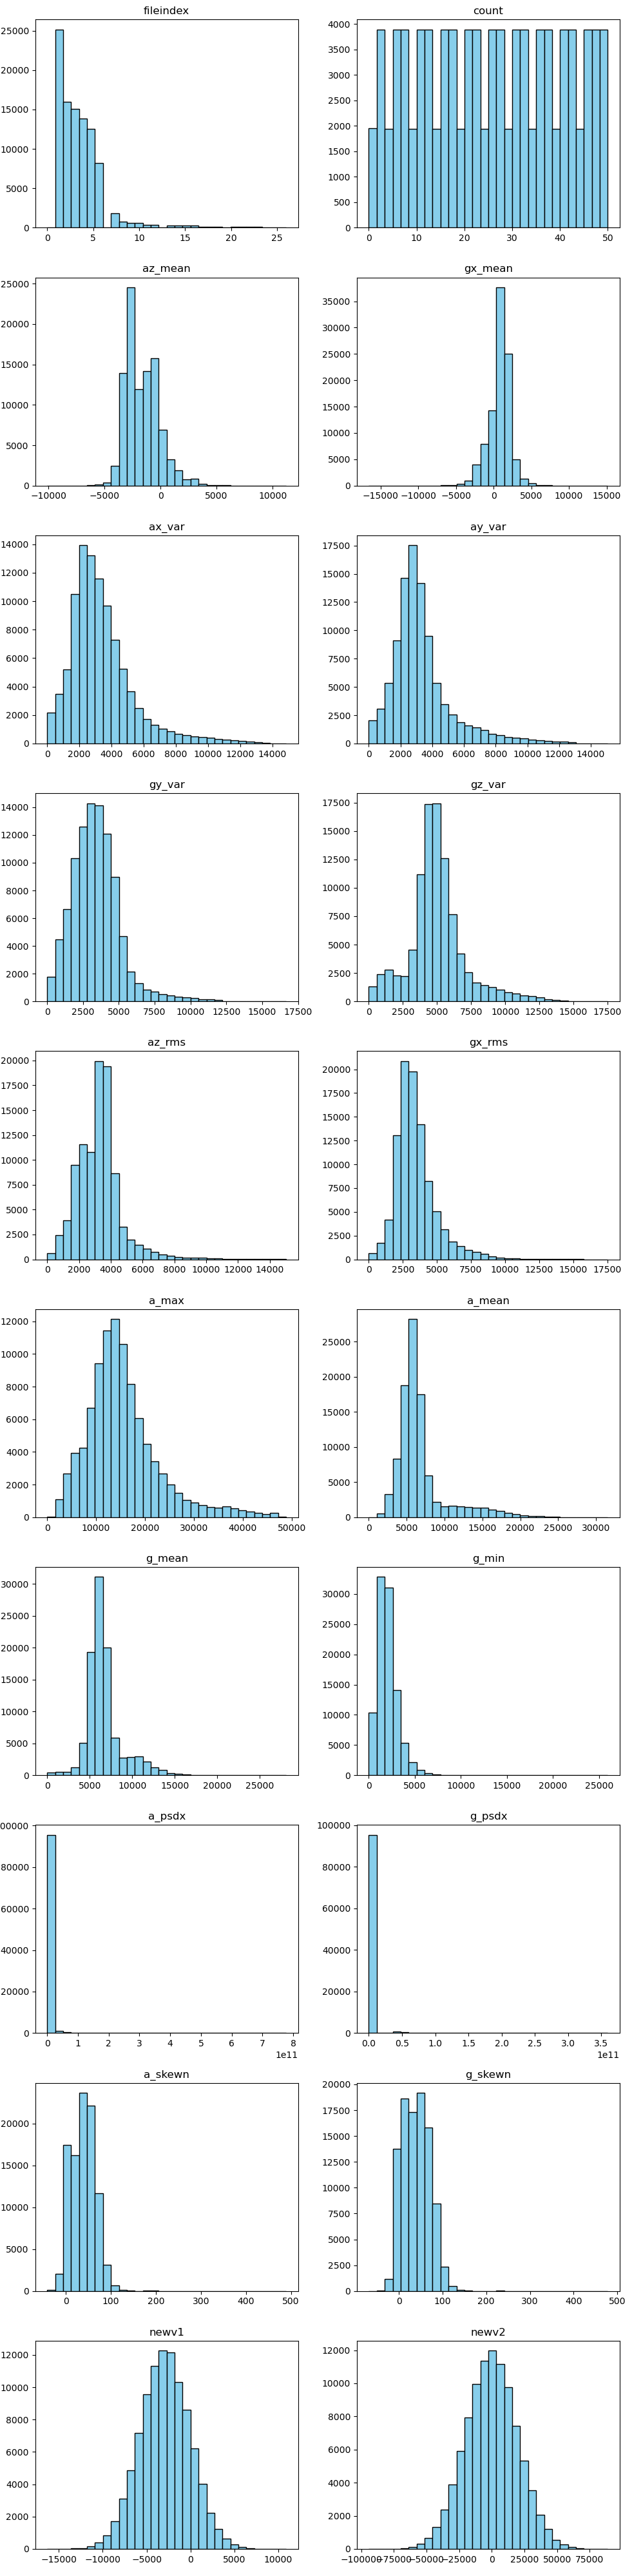
\includegraphics[width=0.85\linewidth, height=0.9\textheight]{distribution_2.png}
    \caption{Distributions of features (2 of 3).}
    \label{fig:distribution-2}
\end{figure}

\begin{figure}[H]
    \centering
    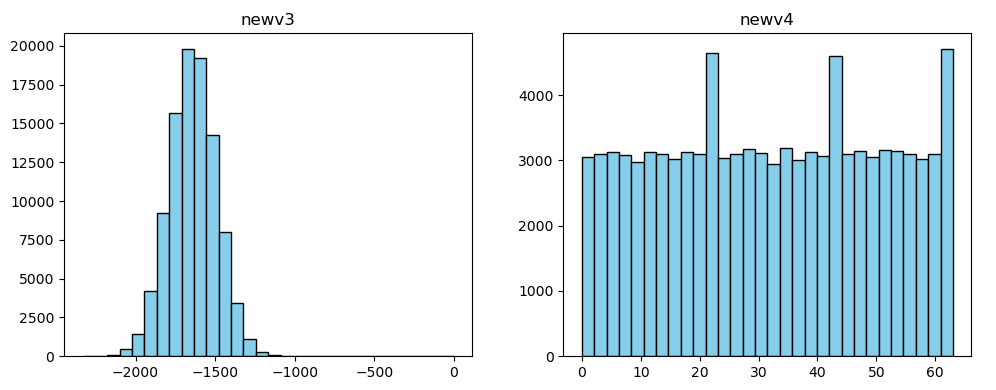
\includegraphics[width=0.85\linewidth]{distribution_3.png}
    \caption{Distributions of features (3 of 3).}
    \label{fig:distribution-3}
\end{figure}







\cite{dryad_tabletennis2021}.

\printbibliography

\end{document}

